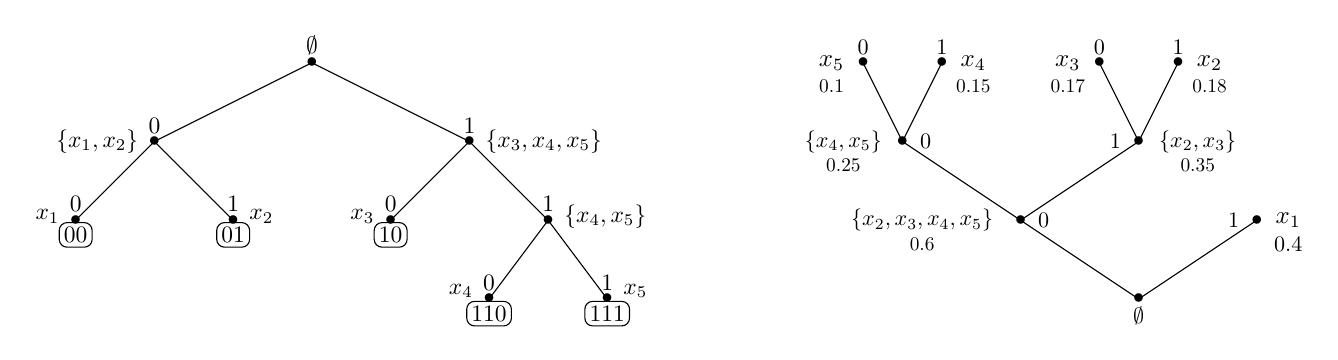
\begin{tikzpicture}%[xscale=3.5,yscale=3]
\shorthandoff{>}
%
% Codigo de Fano
\begin{scope}
\node[scale=.8] at (0,0){$\bullet$};
\node[above,scale=.85] at (0,0){$\emptyset$};
%
% -----
%
\draw (0,0) -- (-2,-1) node[scale=.8]{$\bullet$} node[above,scale=.85]{$0$};
\node[left,scale=.85] at (-2.1,-1){$\{ x_1,x_2\}$};
%
\draw (0,0) -- (2,-1) node[scale=.8]{$\bullet$} node[above,scale=.85]{$1$};
\node[right,scale=.85] at (2.1,-1){$\{ x_3,x_4,x_5\}$};
%
% -----
%
\draw (-2,-1) -- (-3,-2) node[scale=.8]{$\bullet$} node[above,scale=.85]{$0$}
node[inner sep=2pt,outer sep=1pt,draw=black,below,scale=.85,rounded corners=1mm]{$00$};
\node[left,scale=.85] at (-3.1,-1.95){$\boldsymbol{x_1}$};
%
\draw (-2,-1) -- (-1,-2) node[scale=.8]{$\bullet$} node[above,scale=.85]{$1$}
node[inner sep=2pt,outer sep=1pt,draw=black,below,scale=.85,rounded corners=1mm]{$01$};
\node[right,scale=.85] at (-.9,-1.95){$\boldsymbol{x_2}$};
%
\draw (2,-1)-- (1,-2) node[scale=.8]{$\bullet$} node[above,scale=.85]{$0$}
node[inner sep=2pt,outer sep=1pt,draw=black,below,scale=.85,rounded corners=1mm]{$10$};
\node[left,scale=.85] at (.9,-1.95){$\boldsymbol{x_3}$};
%
\draw (2,-1)-- (3,-2) node[scale=.8]{$\bullet$} node[above,scale=.85]{$1$};
\node[right,scale=.85] at (3.1,-1.95){$\{ x_4 , x_5 \}$};
%
% -----
%
\draw (3,-2)-- (2.25,-3) node[scale=.8]{$\bullet$} node[above,scale=.85]{$0$}
node[inner sep=2pt,outer sep=1pt,draw=black,below,scale=.85,rounded corners=1mm]{$110$};
\node[left,scale=.85] at (2.15,-2.9){$\boldsymbol{x_4}$};
%
\draw (3,-2)-- (3.75,-3) node[scale=.8]{$\bullet$} node[above,scale=.85]{$1$}
node[inner sep=2pt,outer sep=1pt,draw=black,below,scale=.85,rounded corners=1mm]{$111$};
\node[right,scale=.85] at (3.85,-2.9){$\boldsymbol{x_5}$};
\end{scope}
%
%
% Codigo de Huffman
\begin{scope}[xshift=12cm]
\draw (-5,0) node[scale=.8]{$\bullet$} node[above,scale=.8]{$0$}
-- (-4.5,-1) node[scale=.8]{$\bullet$} node[right,scale=.8]{$\:\: 0$}
-- (-4,0) node[scale=.8]{$\bullet$} node[above,scale=.8]{$1$};
\node[scale=.9] at (-5.4,0){$\boldsymbol{x_5}$};
\node[scale=.7] at (-5.4,-.3){$0.1$};
\node[scale=.9] at (-3.6,0){$\boldsymbol{x_4}$};
\node[scale=.7] at (-3.6,-.3){$0.15$};
\node[scale=.8] at (-5.25,-1){$\{x_4,x_5\}$};
\node[scale=.7] at (-5.25,-1.3){$0.25$};
%
% -----
%
\draw (-2,0) node[scale=.8]{$\bullet$} node[above,scale=.8]{$0$}
-- (-1.5,-1) node[scale=.8]{$\bullet$} node[left,scale=.8]{$1\:\: $}
-- (-1,0) node[scale=.8]{$\bullet$} node[above,scale=.8]{$1$};
\node[scale=.9] at (-2.4,0){$\boldsymbol{x_3}$};
\node[scale=.7] at (-2.4,-.3){$0.17$};
\node[scale=.9] at (-.6,0){$\boldsymbol{x_2}$};
\node[scale=.7] at (-.6,-.3){$0.18$};
\node[scale=.8] at (-.75,-1){$\{x_2,x_3\}$};
\node[scale=.7] at (-.75,-1.3){$0.35$};
%
% -----
%
\draw (-4.5,-1) -- (-3,-2) node[scale=.8]{$\bullet$} node[right,scale=.8]{$\:\: 0$} -- (-1.5,-1);
\node[scale=.8] at (-4.25,-2){$\{x_2,x_3,x_4,x_5\}$};
\node[scale=.7] at (-4.25,-2.3){$0.6$};
%
% -----
%
\draw (-3,-2) -- (-1.5,-3) node[scale=.8]{$\bullet$} node[below,scale=.8]{$\emptyset$}
-- (0,-2) node[scale=.8]{$\bullet$} node[left,scale=.8]{$1\:\:$};
\node[scale=.9] at (.4,-2){$\boldsymbol{x_1}$};
\node[scale=.8] at (.4,-2.3){$0.4$};
\end{scope}
\end{tikzpicture}
